
\begin{table}[h]
\centering
\caption{Simulation Parameter Values}
\label{table:para2}
\begin{tabular}{|c|ccccccc|}
	\hline
	Parameter     & \textbf{Figure 3}          & \textbf{Figure 4}       & \textbf{Figure 5}    & \textbf{Figure 6}  & \textbf{Figure 7}     & \textbf{Figure 8}    & \textbf{Figure 10}          \\ \hline
	$L$           & $1,3,5,7,10$      & $3$             & $5$         & $5$       & $5$          & $5$         & $3,5,8$            \\ 
	$l_c$         & $0.2,0.3,0.5,0.8$ & $0.3,0.5$       & $0.3$       & $0.2,0.3$ & $0.2,0.3$    & $0.4$       & $0.15,0.2,0.3,0.4$ \\ 
	$\mu_e/\mu_c$ & $100$             & $100$           & $3-300$     & $100$     & $100$        & $100$       & $100$              \\ 
	$\mu_c$       & $0.01$            & $0.01$          & $0.01-0.3$  & $0.01$    & $0.01$       & $0.01$      & $0.01$             \\ 
	$\xi$         & $10,100$          & $5,10,100$      & $1,10,100$  & $10,100$  & $10,100,330$ & $10,100$    & $10,100$           \\ 
	$\upsilon$    & ~                 & ~               & $0.1,0.3,1$ & $0.1,1$   & $0.1,1,3$    & $0.1,1$     & $0.1$              \\ 
	$\phi$        & ~                 & ~               & $0.25$      & $0.5$     & $0.25,0.75$  & $0.25$      & $0.25$             \\ 
	$\tau_r$      & ~                 & $0.1-10^4$      & ~           & ~         & $0.01-10^3$  & $0.01-10^3$ & $10$               \\ 
	$\sigma$      & $0.0002-0.01$     & $0.00003-0.005$ & ~           & ~         & ~            & ~           & ~                  \\
	\hline
\end{tabular}
\end{table}


\begin{figure}[h!]
\centering
\includegraphics[width=\hsize]{active/figures/figure3S}
\caption{\label{fig:passive_supp}  Mechanical properties of passive networks.  \textbf{a)} Elastic modulus of networks.  Our measurements closely match prediction of $G_0\sim\mu/l_c$.  \textbf{b)}  Placeholder for inevitably another figure relevant to passive properties.}
\end{figure}

\begin{figure}[h!]
\centering
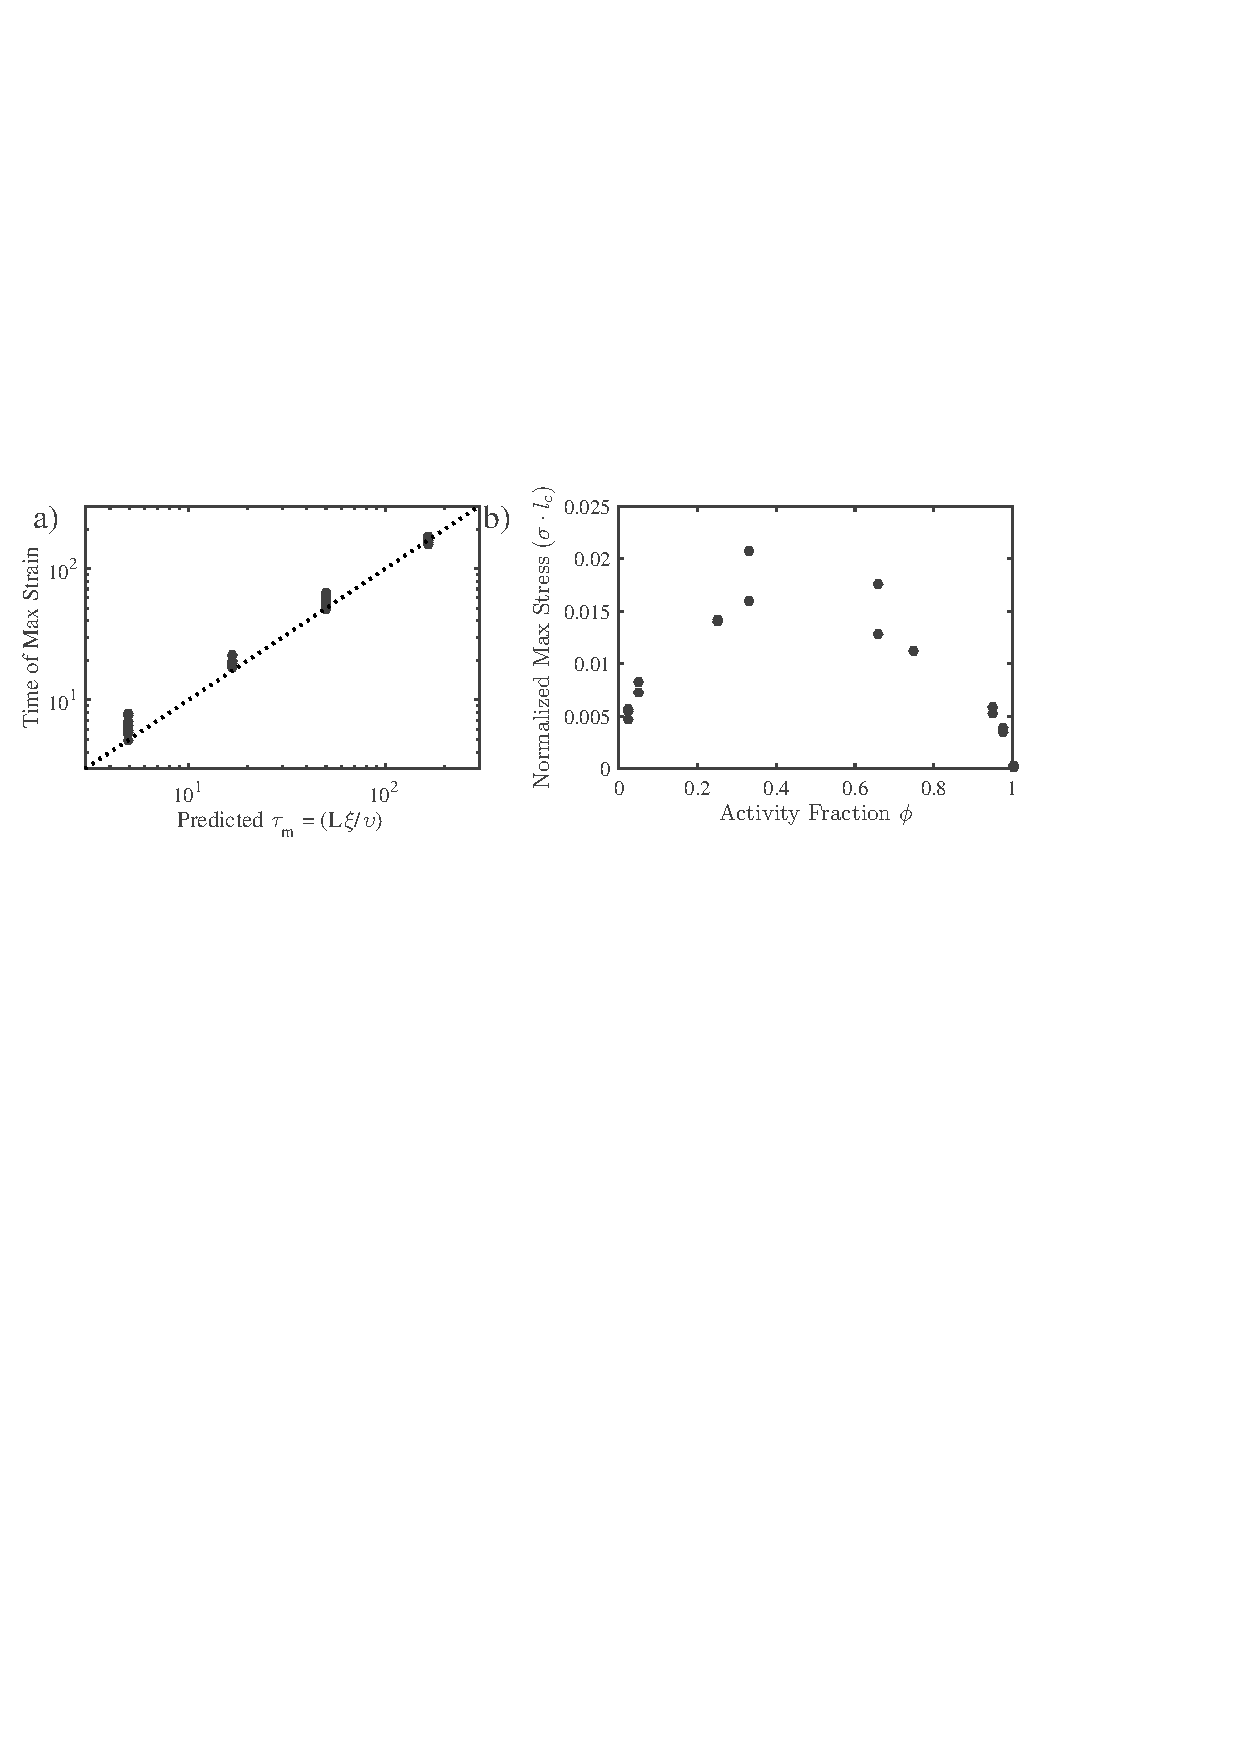
\includegraphics[width=\hsize]{active/figures/figure4S}
\caption{\label{fig:active_supp}  Mechanical properties of active networks.  \textbf{a)}  Timescale of maximum strain in networks free to contract.  This relationship was found phenomenologically.  \textbf{b)}  Dependence of network stress on the fraction of cross-links which are active.  Note that the network stress approaches 0 as $\phi$ approaches 0 or 1.}
\end{figure}

\begin{figure}[h!]
\centering
\includegraphics[width=\hsize]{active/figures/figure5_tear}
\caption{\label{fig:active_supp}  Tearing of active networks is prevented via recycling.  \textbf{a)}  An active network undergoing large scale deformations due to active filament rearrangements.  \textbf{b)}  The same network as in a) but with a shorter filament recycling time.  \textbf{c)}  Time trace of internal stresses for network in panel a.  \textbf{d)}   Time trace of internal stresses for network in panel b.  }
\end{figure}

\begin{figure}[h!]
\centering
\includegraphics[width=\hsize]{active/figures/figure6S}
\caption{\label{fig:combo_prof}  Stress and strain profiles of networks with contractile and passive domains.  \textbf{a)} Blue line indicates strain velocity profile while orange represents net stress as measured in the main text. \textbf{b)} Same as panel a except for the condition where recycling time is 10 s.  Note the increase in net stress and the corresponding increase in flow rate. }
\end{figure}
